
\item A point moves rectilinearly in one direction. Fig. 1.1 shows the distance \( s \) traversed by the point as a function of the time \( t \).
    \begin{center}
        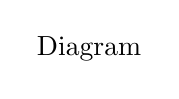
\begin{tikzpicture}
            \node at (0, 0) {Diagram}; % Replace this with the actual TikZ code for the diagram.
        \end{tikzpicture}
    \end{center}
Using the plot find:
\begin{itemize}
    \item the average velocity of the point during the time of motion;
    \item the maximum velocity;
    \item the time moment \( t_0 \) at which the instantaneous velocity is equal to the mean velocity averaged over the first \( t_0 \) seconds.
\end{itemize}

\begin{solution}
    \begin{center}
        \begin{tikzpicture}
            \pic at (0, 0) {frame=3cm};
        \end{tikzpicture}
    \end{center}
    
    \begin{align*}
        \intertext{\textbf{1.4 (a)} Sought average velocity}
        <v> &= \dfrac{s}{t} = \dfrac{200 \text{ cm}}{20 \text{ s}} = 10 \text{ cm/s}\\
        \intertext{\textbf{(b)} For the maximum velocity, $ds/dt$ should be maximum. From the figure $ds/dt$ is maximum for all points on the line $ab$ thus the sought maximum velocity becomes average velocity for the line $ab$ and is}
        &= \dfrac{100 \text{ cm}}{4 \text{ s}} = 25 \text{ cm/s}\\
        \intertext{\textbf{(c)} Time $t_0$ should be such that corresponding to it the slope $ds/dt$ should coincide with the chord $Oc$, to satisfy the relationship $ds/dt = s/t_0$. From figure the tangent at point $c$ passes through the origin and thus corresponding time $t = t_0 = 16 \text{ s}$.}
    \end{align*}
\end{solution}
